%%%%%%%%%%%%%%%%%%%%%%%%%%%%%%%%%%%%%%%%%
% The Legrand Orange Book
% LaTeX Template
% Version 2.0 (9/2/15)
%
% This template has been downloaded from:
% http://www.LaTeXTemplates.com
%
% Mathias Legrand (legrand.mathias@gmail.com) with modifications by:
% Vel (vel@latextemplates.com)
%
% License:
% CC BY-NC-SA 3.0 (http://creativecommons.org/licenses/by-nc-sa/3.0/)
%
% Compiling this template:
% This template uses biber for its bibliography and makeindex for its index.
% When you first open the template, compile it from the command line with the 
% commands below to make sure your LaTeX distribution is configured correctly:
%
% 1) pdflatex main
% 2) makeindex main.idx -s StyleInd.ist
% 3) biber main
% 4) pdflatex main x 2
%
% After this, when you wish to update the bibliography/index use the appropriate
% command above and make sure to compile with pdflatex several times 
% afterwards to propagate your changes to the document.
%
% This template also uses a number of packages which may need to be
% updated to the newest versions for the template to compile. It is strongly
% recommended you update your LaTeX distribution if you have any
% compilation errors.
%
% Important note:
% Chapter heading images should have a 2:1 width:height ratio,
% e.g. 920px width and 460px height.
%
%%%%%%%%%%%%%%%%%%%%%%%%%%%%%%%%%%%%%%%%%

%----------------------------------------------------------------------------------------
%	PACKAGES AND OTHER DOCUMENT CONFIGURATIONS
%----------------------------------------------------------------------------------------

\documentclass[11pt,fleqn]{book} % Default font size and left-justified equations

%----------------------------------------------------------------------------------------

%%%%%%%%%%%%%%%%%%%%%%%%%%%%%%%%%%%%%%%%%
% The Legrand Orange Book
% Structural Definitions File
% Version 2.0 (9/2/15)
%
% Original author:
% Mathias Legrand (legrand.mathias@gmail.com) with modifications by:
% Vel (vel@latextemplates.com)
% 
% This file has been downloaded from:
% http://www.LaTeXTemplates.com
%
% License:
% CC BY-NC-SA 3.0 (http://creativecommons.org/licenses/by-nc-sa/3.0/)
%
%%%%%%%%%%%%%%%%%%%%%%%%%%%%%%%%%%%%%%%%%

%----------------------------------------------------------------------------------------
%	VARIOUS REQUIRED PACKAGES AND CONFIGURATIONS
%----------------------------------------------------------------------------------------

\usepackage[top=3cm,bottom=3cm,left=3cm,right=3cm,headsep=10pt,a4paper]{geometry} % Page margins

\usepackage{graphicx} % Required for including pictures
\graphicspath{{Pictures/}} % Specifies the directory where pictures are stored

\usepackage{lipsum} % Inserts dummy text

\usepackage{tikz} % Required for drawing custom shapes

\usepackage[english]{babel} % English language/hyphenation

\usepackage{enumitem} % Customize lists
\setlist{nolistsep} % Reduce spacing between bullet points and numbered lists

\usepackage{booktabs} % Required for nicer horizontal rules in tables

\usepackage{xcolor} % Required for specifying colors by name
\definecolor{ocre}{RGB}{43,157,209} % Define the orange color used for highlighting throughout the book

%----------------------------------------------------------------------------------------
%	FONTS
%----------------------------------------------------------------------------------------

\usepackage{avant} % Use the Avantgarde font for headings
%\usepackage{times} % Use the Times font for headings
\usepackage{mathptmx} % Use the Adobe Times Roman as the default text font together with math symbols from the Sym­bol, Chancery and Com­puter Modern fonts

\usepackage{microtype} % Slightly tweak font spacing for aesthetics
\usepackage[utf8x]{inputenc} % Required for including letters with accents
\usepackage[T1]{fontenc} % Use 8-bit encoding that has 256 glyphs
\usepackage{textcomp}
\usepackage{eurosans}
%----------------------------------------------------------------------------------------
%	BIBLIOGRAPHY AND INDEX
%----------------------------------------------------------------------------------------

\usepackage[style=alphabetic,citestyle=numeric,sorting=nyt,sortcites=true,autopunct=true,babel=hyphen,hyperref=true,abbreviate=false,backref=true,backend=biber]{biblatex}
\addbibresource{bibliography.bib} % BibTeX bibliography file
\defbibheading{bibempty}{}

\usepackage{calc} % For simpler calculation - used for spacing the index letter headings correctly
\usepackage{makeidx} % Required to make an index
\makeindex % Tells LaTeX to create the files required for indexing

%----------------------------------------------------------------------------------------
%	MAIN TABLE OF CONTENTS
%----------------------------------------------------------------------------------------

\usepackage{titletoc} % Required for manipulating the table of contents

\contentsmargin{0cm} % Removes the default margin

% Part text styling
\titlecontents{part}[0cm]
{\addvspace{20pt}\centering\large\bfseries}
{}
{}
{}

% Chapter text styling
\titlecontents{chapter}[1.25cm] % Indentation
{\addvspace{12pt}\large\sffamily\bfseries} % Spacing and font options for chapters
{\color{ocre!60}\contentslabel[\Large\thecontentslabel]{1.25cm}\color{ocre}} % Chapter number
{\color{ocre}}  
{\color{ocre!60}\normalsize\;\titlerule*[.5pc]{.}\;\thecontentspage} % Page number

% Section text styling
\titlecontents{section}[1.25cm] % Indentation
{\addvspace{3pt}\sffamily\bfseries} % Spacing and font options for sections
{\contentslabel[\thecontentslabel]{1.25cm}} % Section number
{}
{\hfill\color{black}\thecontentspage} % Page number
[]

% Subsection text styling
\titlecontents{subsection}[1.25cm] % Indentation
{\addvspace{1pt}\sffamily\small} % Spacing and font options for subsections
{\contentslabel[\thecontentslabel]{1.25cm}} % Subsection number
{}
{\ \titlerule*[.5pc]{.}\;\thecontentspage} % Page number
[]

% List of figures
\titlecontents{figure}[0em]
{\addvspace{-5pt}\sffamily}
{\thecontentslabel\hspace*{1em}}
{}
{\ \titlerule*[.5pc]{.}\;\thecontentspage}
[]

% List of tables
\titlecontents{table}[0em]
{\addvspace{-5pt}\sffamily}
{\thecontentslabel\hspace*{1em}}
{}
{\ \titlerule*[.5pc]{.}\;\thecontentspage}
[]

%----------------------------------------------------------------------------------------
%	MINI TABLE OF CONTENTS IN PART HEADS
%----------------------------------------------------------------------------------------

% Chapter text styling
\titlecontents{lchapter}[0em] % Indenting
{\addvspace{15pt}\large\sffamily\bfseries} % Spacing and font options for chapters
{\color{ocre}\contentslabel[\Large\thecontentslabel]{1.25cm}\color{ocre}} % Chapter number
{}  
{\color{ocre}\normalsize\sffamily\bfseries\;\titlerule*[.5pc]{.}\;\thecontentspage} % Page number

% Section text styling
\titlecontents{lsection}[0em] % Indenting
{\sffamily\small} % Spacing and font options for sections
{\contentslabel[\thecontentslabel]{1.25cm}} % Section number
{}
{}

% Subsection text styling
\titlecontents{lsubsection}[.5em] % Indentation
{\normalfont\footnotesize\sffamily} % Font settings
{}
{}
{}

%----------------------------------------------------------------------------------------
%	PAGE HEADERS
%----------------------------------------------------------------------------------------

\usepackage{fancyhdr} % Required for header and footer configuration

\pagestyle{fancy}
\renewcommand{\chaptermark}[1]{\markboth{\sffamily\normalsize\bfseries\chaptername\ \thechapter.\ #1}{}} % Chapter text font settings
\renewcommand{\sectionmark}[1]{\markright{\sffamily\normalsize\thesection\hspace{5pt}#1}{}} % Section text font settings
\fancyhf{} \fancyhead[LE,RO]{\sffamily\normalsize} % Font setting for the page number in the header
\fancyhead[LO]{\rightmark} % Print the nearest section name on the left side of odd pages
\fancyhead[RE]{\leftmark} % Print the current chapter name on the right side of even pages
\renewcommand{\headrulewidth}{1pt} % Width of the rule under the header
\addtolength{\headheight}{2.5pt} % Increase the spacing around the header slightly
\renewcommand{\footrulewidth}{0pt} % Removes the rule in the footer
\fancypagestyle{plain}{\fancyhead{}\renewcommand{\headrulewidth}{0pt}} % Style for when a plain pagestyle is specified

%------ FOOTER ------%
\fancyfoot[RE,RO]{\thepage}
\fancyfoot[LE,LO]{Projet MI44}
\renewcommand{\footrulewidth}{0.5pt}

% Removes the header from odd empty pages at the end of chapters
\makeatletter
\renewcommand{\cleardoublepage}{
\clearpage\ifodd\c@page\else
\hbox{}
\vspace*{\fill}
\thispagestyle{empty}
\newpage
\fi}

%----------------------------------------------------------------------------------------
%	THEOREM STYLES
%----------------------------------------------------------------------------------------

\usepackage{amsmath,amsfonts,amssymb,amsthm} % For math equations, theorems, symbols, etc

\newcommand{\intoo}[2]{\mathopen{]}#1\,;#2\mathclose{[}}
\newcommand{\ud}{\mathop{\mathrm{{}d}}\mathopen{}}
\newcommand{\intff}[2]{\mathopen{[}#1\,;#2\mathclose{]}}
\newtheorem{notation}{Notation}[chapter]

% Boxed/framed environments
\newtheoremstyle{ocrenumbox}% % Theorem style name
{0pt}% Space above
{0pt}% Space below
{\normalfont}% % Body font
{}% Indent amount
{\small\bf\sffamily\color{ocre}}% % Theorem head font
{\;}% Punctuation after theorem head
{0.25em}% Space after theorem head
{\small\sffamily\color{ocre}\thmname{#1}\nobreakspace\thmnumber{\@ifnotempty{#1}{}\@upn{#2}}% Theorem text (e.g. Theorem 2.1)
\thmnote{\nobreakspace\the\thm@notefont\sffamily\bfseries\color{black}---\nobreakspace#3.}} % Optional theorem note
\renewcommand{\qedsymbol}{$\blacksquare$}% Optional qed square

\newtheoremstyle{blacknumex}% Theorem style name
{5pt}% Space above
{5pt}% Space below
{\normalfont}% Body font
{} % Indent amount
{\small\bf\sffamily}% Theorem head font
{\;}% Punctuation after theorem head
{0.25em}% Space after theorem head
{\small\sffamily{\tiny\ensuremath{\blacksquare}}\nobreakspace\thmname{#1}\nobreakspace\thmnumber{\@ifnotempty{#1}{}\@upn{#2}}% Theorem text (e.g. Theorem 2.1)
\thmnote{\nobreakspace\the\thm@notefont\sffamily\bfseries---\nobreakspace#3.}}% Optional theorem note

\newtheoremstyle{blacknumbox} % Theorem style name
{0pt}% Space above
{0pt}% Space below
{\normalfont}% Body font
{}% Indent amount
{\small\bf\sffamily}% Theorem head font
{\;}% Punctuation after theorem head
{0.25em}% Space after theorem head
{\small\sffamily\thmname{#1}\nobreakspace\thmnumber{\@ifnotempty{#1}{}\@upn{#2}}% Theorem text (e.g. Theorem 2.1)
\thmnote{\nobreakspace\the\thm@notefont\sffamily\bfseries---\nobreakspace#3.}}% Optional theorem note

% Non-boxed/non-framed environments
\newtheoremstyle{ocrenum}% % Theorem style name
{5pt}% Space above
{5pt}% Space below
{\normalfont}% % Body font
{}% Indent amount
{\small\bf\sffamily\color{ocre}}% % Theorem head font
{\;}% Punctuation after theorem head
{0.25em}% Space after theorem head
{\small\sffamily\color{ocre}\thmname{#1}\nobreakspace\thmnumber{\@ifnotempty{#1}{}\@upn{#2}}% Theorem text (e.g. Theorem 2.1)
\thmnote{\nobreakspace\the\thm@notefont\sffamily\bfseries\color{black}---\nobreakspace#3.}} % Optional theorem note
\renewcommand{\qedsymbol}{$\blacksquare$}% Optional qed square
\makeatother

% Defines the theorem text style for each type of theorem to one of the three styles above
\newcounter{dummy} 
\numberwithin{dummy}{section}
\theoremstyle{ocrenumbox}
\newtheorem{theoremeT}[dummy]{Theorem}
\newtheorem{problem}{Problem}[chapter]
\newtheorem{exerciseT}{Exercise}[chapter]
\theoremstyle{blacknumex}
\newtheorem{exampleT}{Example}[chapter]
\theoremstyle{blacknumbox}
\newtheorem{vocabulary}{Vocabulary}[chapter]
\newtheorem{definitionT}{Definition}[section]
\newtheorem{corollaryT}[dummy]{Corollary}
\theoremstyle{ocrenum}
\newtheorem{proposition}[dummy]{Proposition}

%----------------------------------------------------------------------------------------
%	DEFINITION OF COLORED BOXES
%----------------------------------------------------------------------------------------

\RequirePackage[framemethod=default]{mdframed} % Required for creating the theorem, definition, exercise and corollary boxes

% Theorem box
\newmdenv[skipabove=7pt,
skipbelow=7pt,
backgroundcolor=black!5,
linecolor=ocre,
innerleftmargin=5pt,
innerrightmargin=5pt,
innertopmargin=5pt,
leftmargin=0cm,
rightmargin=0cm,
innerbottommargin=5pt]{tBox}

% Exercise box	  
\newmdenv[skipabove=7pt,
skipbelow=7pt,
rightline=false,
leftline=true,
topline=false,
bottomline=false,
backgroundcolor=ocre!10,
linecolor=ocre,
innerleftmargin=5pt,
innerrightmargin=5pt,
innertopmargin=5pt,
innerbottommargin=5pt,
leftmargin=0cm,
rightmargin=0cm,
linewidth=4pt]{eBox}	

% Definition box
\newmdenv[skipabove=7pt,
skipbelow=7pt,
rightline=false,
leftline=true,
topline=false,
bottomline=false,
linecolor=ocre,
innerleftmargin=5pt,
innerrightmargin=5pt,
innertopmargin=0pt,
leftmargin=0cm,
rightmargin=0cm,
linewidth=4pt,
innerbottommargin=0pt]{dBox}	

% Corollary box
\newmdenv[skipabove=7pt,
skipbelow=7pt,
rightline=false,
leftline=true,
topline=false,
bottomline=false,
linecolor=gray,
backgroundcolor=black!5,
innerleftmargin=5pt,
innerrightmargin=5pt,
innertopmargin=5pt,
leftmargin=0cm,
rightmargin=0cm,
linewidth=4pt,
innerbottommargin=5pt]{cBox}

% Creates an environment for each type of theorem and assigns it a theorem text style from the "Theorem Styles" section above and a colored box from above
\newenvironment{theorem}{\begin{tBox}\begin{theoremeT}}{\end{theoremeT}\end{tBox}}
\newenvironment{exercise}{\begin{eBox}\begin{exerciseT}}{\hfill{\color{ocre}\tiny\ensuremath{\blacksquare}}\end{exerciseT}\end{eBox}}				  
\newenvironment{definition}{\begin{dBox}\begin{definitionT}}{\end{definitionT}\end{dBox}}	
\newenvironment{example}{\begin{exampleT}}{\hfill{\tiny\ensuremath{\blacksquare}}\end{exampleT}}		
\newenvironment{corollary}{\begin{cBox}\begin{corollaryT}}{\end{corollaryT}\end{cBox}}	

%----------------------------------------------------------------------------------------
%	REMARK ENVIRONMENT
%----------------------------------------------------------------------------------------

\newenvironment{remark}{\par\vspace{10pt}\small % Vertical white space above the remark and smaller font size
\begin{list}{}{
\leftmargin=35pt % Indentation on the left
\rightmargin=25pt}\item\ignorespaces % Indentation on the right
\makebox[-2.5pt]{\begin{tikzpicture}[overlay]
\node[draw=ocre!60,line width=1pt,circle,fill=ocre!25,font=\sffamily\bfseries,inner sep=2pt,outer sep=0pt] at (-15pt,0pt){\textcolor{ocre}{R}};\end{tikzpicture}} % Orange R in a circle
\advance\baselineskip -1pt}{\end{list}\vskip5pt} % Tighter line spacing and white space after remark

%----------------------------------------------------------------------------------------
%	SECTION NUMBERING IN THE MARGIN
%----------------------------------------------------------------------------------------

\makeatletter
\renewcommand{\@seccntformat}[1]{\llap{\textcolor{ocre}{\csname the#1\endcsname}\hspace{1em}}}                    
\renewcommand{\section}{\@startsection{section}{1}{\z@}
{-4ex \@plus -1ex \@minus -.4ex}
{1ex \@plus.2ex }
{\normalfont\large\sffamily\bfseries}}
\renewcommand{\subsection}{\@startsection {subsection}{2}{\z@}
{-3ex \@plus -0.1ex \@minus -.4ex}
{0.5ex \@plus.2ex }
{\normalfont\sffamily\bfseries}}
\renewcommand{\subsubsection}{\@startsection {subsubsection}{3}{\z@}
{-2ex \@plus -0.1ex \@minus -.2ex}
{.2ex \@plus.2ex }
{\normalfont\small\sffamily\bfseries}}                        
\renewcommand\paragraph{\@startsection{paragraph}{4}{\z@}
{-2ex \@plus-.2ex \@minus .2ex}
{.1ex}
{\normalfont\small\sffamily\bfseries}}

%----------------------------------------------------------------------------------------
%	PART HEADINGS
%----------------------------------------------------------------------------------------

% numbered part in the table of contents
\newcommand{\@mypartnumtocformat}[2]{%
\setlength\fboxsep{0pt}%
\noindent\colorbox{ocre!20}{\strut\parbox[c][.7cm]{\ecart}{\color{ocre!70}\Large\sffamily\bfseries\centering#1}}\hskip\esp\colorbox{ocre!40}{\strut\parbox[c][.7cm]{\linewidth-\ecart-\esp}{\Large\sffamily\centering#2}}}%
%%%%%%%%%%%%%%%%%%%%%%%%%%%%%%%%%%
% unnumbered part in the table of contents
\newcommand{\@myparttocformat}[1]{%
\setlength\fboxsep{0pt}%
\noindent\colorbox{ocre!40}{\strut\parbox[c][.7cm]{\linewidth}{\Large\sffamily\centering#1}}}%
%%%%%%%%%%%%%%%%%%%%%%%%%%%%%%%%%%
\newlength\esp
\setlength\esp{4pt}
\newlength\ecart
\setlength\ecart{1.2cm-\esp}
\newcommand{\thepartimage}{}%
\newcommand{\partimage}[1]{\renewcommand{\thepartimage}{#1}}%
\def\@part[#1]#2{%
\ifnum \c@secnumdepth >-2\relax%
\refstepcounter{part}%
\addcontentsline{toc}{part}{\texorpdfstring{\protect\@mypartnumtocformat{\thepart}{#1}}{\partname~\thepart\ ---\ #1}}
\else%
\addcontentsline{toc}{part}{\texorpdfstring{\protect\@myparttocformat{#1}}{#1}}%
\fi%
\startcontents%
\markboth{}{}%
{\thispagestyle{empty}%
\begin{tikzpicture}[remember picture,overlay]%
\node at (current page.north west){\begin{tikzpicture}[remember picture,overlay]%	
\fill[ocre!20](0cm,0cm) rectangle (\paperwidth,-\paperheight);
\node[anchor=north] at (4cm,-3.25cm){\color{ocre!40}\fontsize{220}{100}\sffamily\bfseries\@Roman\c@part}; 
\node[anchor=south east] at (\paperwidth-1cm,-\paperheight+1cm){\parbox[t][][t]{8.5cm}{
\printcontents{l}{0}{\setcounter{tocdepth}{1}}%
}};
\node[anchor=north east] at (\paperwidth-1.5cm,-3.25cm){\parbox[t][][t]{15cm}{\strut\raggedleft\color{white}\fontsize{30}{30}\sffamily\bfseries#2}};
\end{tikzpicture}};
\end{tikzpicture}}%
\@endpart}
\def\@spart#1{%
\startcontents%
\phantomsection
{\thispagestyle{empty}%
\begin{tikzpicture}[remember picture,overlay]%
\node at (current page.north west){\begin{tikzpicture}[remember picture,overlay]%	
\fill[ocre!20](0cm,0cm) rectangle (\paperwidth,-\paperheight);
\node[anchor=north east] at (\paperwidth-1.5cm,-3.25cm){\parbox[t][][t]{15cm}{\strut\raggedleft\color{white}\fontsize{30}{30}\sffamily\bfseries#1}};
\end{tikzpicture}};
\end{tikzpicture}}
\addcontentsline{toc}{part}{\texorpdfstring{%
\setlength\fboxsep{0pt}%
\noindent\protect\colorbox{ocre!40}{\strut\protect\parbox[c][.7cm]{\linewidth}{\Large\sffamily\protect\centering #1\quad\mbox{}}}}{#1}}%
\@endpart}
\def\@endpart{\vfil\newpage
\if@twoside
\if@openright
\null
\thispagestyle{empty}%
\newpage
\fi
\fi
\if@tempswa
\twocolumn
\fi}

%----------------------------------------------------------------------------------------
%	CHAPTER HEADINGS
%----------------------------------------------------------------------------------------

\newcommand{\thechapterimage}{}%
\newcommand{\chapterimage}[1]{\renewcommand{\thechapterimage}{#1}}%
\def\@makechapterhead#1{%
{\parindent \z@ \raggedright \normalfont
\ifnum \c@secnumdepth >\m@ne
\if@mainmatter
\begin{tikzpicture}[remember picture,overlay]
\node at (current page.north west)
{\begin{tikzpicture}[remember picture,overlay]
\node[anchor=north west,inner sep=0pt] at (0,0) {\includegraphics[width=\paperwidth]{\thechapterimage}};
\draw[anchor=west] (\Gm@lmargin,-9cm) node [line width=2pt,rounded corners=15pt,draw=ocre,fill=white,fill opacity=0.5,inner sep=15pt]{\strut\makebox[22cm]{}};
\draw[anchor=west] (\Gm@lmargin+.3cm,-9cm) node {\huge\sffamily\bfseries\color{black}\thechapter. #1\strut};
\end{tikzpicture}};
\end{tikzpicture}
\else
\begin{tikzpicture}[remember picture,overlay]
\node at (current page.north west)
{\begin{tikzpicture}[remember picture,overlay]
\node[anchor=north west,inner sep=0pt] at (0,0) {\includegraphics[width=\paperwidth]{\thechapterimage}};
\draw[anchor=west] (\Gm@lmargin,-9cm) node [line width=2pt,rounded corners=15pt,draw=ocre,fill=white,fill opacity=0.5,inner sep=15pt]{\strut\makebox[22cm]{}};
\draw[anchor=west] (\Gm@lmargin+.3cm,-9cm) node {\huge\sffamily\bfseries\color{black}#1\strut};
\end{tikzpicture}};
\end{tikzpicture}
\fi\fi\par\vspace*{270\p@}}}

%-------------------------------------------

\def\@makeschapterhead#1{%
\begin{tikzpicture}[remember picture,overlay]
\node at (current page.north west)
{\begin{tikzpicture}[remember picture,overlay]
\node[anchor=north west,inner sep=0pt] at (0,0) {\includegraphics[width=\paperwidth]{\thechapterimage}};
\draw[anchor=west] (\Gm@lmargin,-9cm) node [line width=2pt,rounded corners=15pt,draw=ocre,fill=white,fill opacity=0.5,inner sep=15pt]{\strut\makebox[22cm]{}};
\draw[anchor=west] (\Gm@lmargin+.3cm,-9cm) node {\huge\sffamily\bfseries\color{black}#1\strut};
\end{tikzpicture}};
\end{tikzpicture}
\par\vspace*{270\p@}}
\makeatother

%----------------------------------------------------------------------------------------
%	HYPERLINKS IN THE DOCUMENTS
%----------------------------------------------------------------------------------------

\usepackage{hyperref}
\hypersetup{hidelinks,backref=true,pagebackref=true,hyperindex=true,colorlinks=false,breaklinks=true,urlcolor= ocre,bookmarks=true,bookmarksopen=false,pdftitle={Title},pdfauthor={Author}}
\usepackage{bookmark}
\bookmarksetup{
open,
numbered,
addtohook={%
\ifnum\bookmarkget{level}=0 % chapter
\bookmarksetup{bold}%
\fi
\ifnum\bookmarkget{level}=-1 % part
\bookmarksetup{color=ocre,bold}%
\fi
}
} % Insert the commands.tex file which contains the majority of the structure behind the template
\begin{document}

%----------------------------------------------------------------------------------------
%	TITLE PAGE
%----------------------------------------------------------------------------------------

\begingroup
\thispagestyle{empty}
\begin{tikzpicture}[remember picture,overlay]
\coordinate [below=12cm] (midpoint) at (current page.north);
\node at (current page.north west)
{\begin{tikzpicture}[remember picture,overlay]
\node[anchor=north west,inner sep=0pt] at (0,0) {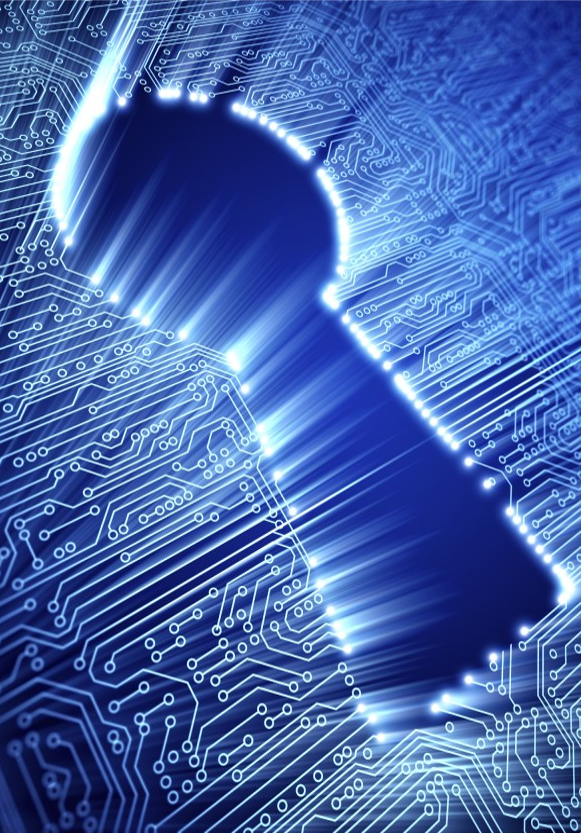
\includegraphics[width=\paperwidth]{crypto}}; % Background image
\draw[anchor=north] (midpoint) node [fill=ocre!30!white,fill opacity=0.6,text opacity=1,inner sep=1cm]{\Huge\centering\bfseries\sffamily\parbox[c][][t]{\paperwidth}{\centering Projet MI44\\[15pt] % Book title
{\huge DAUDAN Florian / GUIMARAES Patrick}}}; % Author name
\end{tikzpicture}};
\end{tikzpicture}
\vfill
\endgroup

%----------------------------------------------------------------------------------------
%	TABLE OF CONTENTS
%----------------------------------------------------------------------------------------

\renewcommand*\contentsname{Sommaire}

\chapterimage{crypto_chapter} % Table of contents heading image

\pagestyle{empty} % No headers

\tableofcontents % Print the table of contents itself

%\cleardoublepage % Forces the first chapter to start on an odd page so it's on the right

%\pagestyle{fancy} % Print headers again

%----------------------------------------------------------------------------------------
%	PART
%----------------------------------------------------------------------------------------

%\part{Part One}

%----------------------------------------------------------------------------------------
%	CHAPTER 1
%----------------------------------------------------------------------------------------
\cleardoublepage
\chapterimage{crypto_chapter} % Chapter heading image

\chapter{TP1 : Cryptographie par bloc}

%\section{Paragraphs of Text}\index{Paragraphs of Text}

%\lipsum[1-7] % Dummy text
%------------------------------------------------

\section{Introduction}

\paragraph{}Afin de gérer la conversion d'un caractère en un nombre binaire, nous avons mis au point un dictionnaire. En effet, chaque caractère (A,B,C…) correspond à un nombre (A=0, B=1,C=2,…) et le dictionnaire va donc permettre d'attribuer plus rapidement un nombre à un caractère. Et dans le cadre inverse, un second dictionnaire va permettre de passer d'un nombre au caractère correspondant.
\vspace{0.5cm} Nous avons 32 caractères à gérer ; toutes les lettres de l'alphabet latin ainsi que les caractères espace, point, virgule, apostrophe, point d'exclamation et point d'interrogation. Ce qui nous fait un total de 32 caractère codable sur 5 bits en binaire. Notons la constante NB\_BIT permettant d'ajuster le codage des caractères. En outre, elle permet d’égaliser l'écriture de tous les nombres binaires qui auront, de surcroît, le même nombre de bit. Par exemple, B (=1) sera écrit 00001.
%------------------------------------------------

\section{Binaire}\index{Binaire}

\subsection{Chiffrer}\index{Crypter}
%Texte encrypt \cite{image_crypt}.
\paragraph{}La fonction \textbf{encrypt\_binaire(lettre)} reçoit en paramètre un caractère et retourne directement le nombre binaire associé. En prime abord, elle demande au dictionnaire de lui retourner la valeur numérique en base 10 du caractère . Puis ensuite elle convertit cette valeur en binaire qui sera elle-même envoyée à la fonction \textbf{toilettage\_binaire(binaire)} qui, comme son nom l'indique, va se charger d'écrire le binaire sous le bon nombre de bit(cf. constante NB\_BIT).
Une fois ces opérations terminées, le caractère en binaire sera renvoyé.
\vspace{0.5cm}Dans la même optique, nous avons conçu la fonction \textbf{encrypt\_mot\_binaire(mot)}  qui va recevoir un mot, ou une phrase, et renvoyer directement le mot/phrase converti(e). 

\begin{figure}[!h]
\centering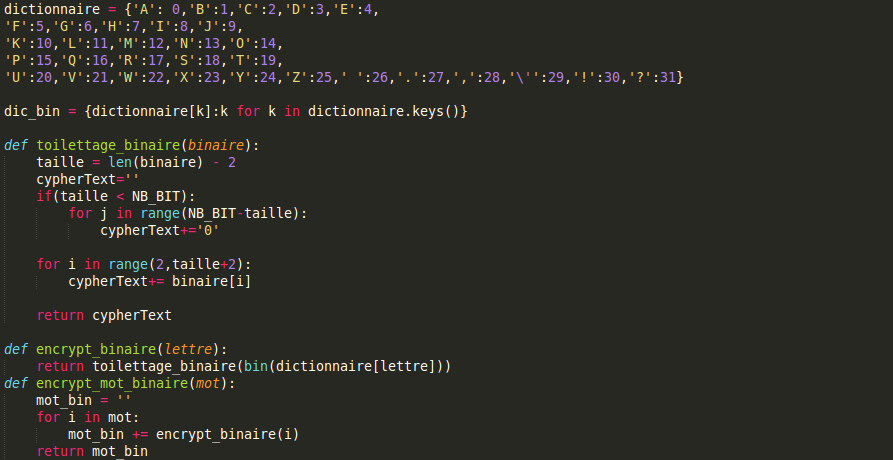
\includegraphics[scale=0.5]{encrypt_bin}
\caption{Fonctions de conversion en binaire}

\end{figure}


%------------------------------------------------
\subsection{Déchiffrer}\index{Decrypter}

\paragraph{}Finalement, pour réaliser l'opération inverse, c'est à dire de convertir un binaire en caractère, nous avons écrit la fonction \textbf{decrypt\_binaire()} qui reçoit un nombre binaire. Cette méthode va en premier lieu convertir le nombre en décimal. Puis appeler le second dictionnaire pour lui demander quel caractère est associé au nombre. Enfin, elle va retourner le caractère trouvé. De façon similaire à encryp\_mot\_binaire(), nous avons écrit \textbf{decrypt\_mot\_binaire(}) qui à partir d'une phrase ou un mot binaire de taille \% NB\_BIT, va retourner les caractères correspondant.

\begin{figure}[!h]
\centering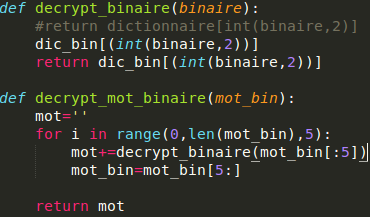
\includegraphics[scale=0.5]{decrypt_binaire}
\caption{Fonctions de conversion en caractère}
\label{fig:nonfloat}
\end{figure}

%------------------------------------------------

\subsection{Ou Exclusif}\index{Ou Exclusif}

\paragraph{}La fonction \textbf{ouExclusif(A,B)} réalise le ou exclusif en binaire, elle prend en compte deux binaires.
\vspace{0.5cm}On parcourt le premier binaire bit à bit, on compare le bit avec le bit de l'autre binaire. S'ils sont égals et que l'un d'eux est égal à 1, on retourne 0. Sinon si l'un deux est égal à 1 on retourne 1. Dans les autres cas on retourne 0. Une fois terminé, nous avons le résultat de l'addition binaire.

\begin{figure}[!h]
\centering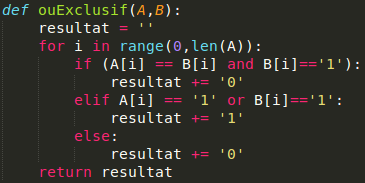
\includegraphics[scale=0.5]{ouExclusif}
\caption{ou exclusif(XOR)}
\end{figure}

%------------------------------------------------

\section{Function}\index{Function}

\paragraph{}La fonction \textbf{function()} prend en paramètre un message msg de 2 caractères ainsi qu'une clé Key de 2 caractères convertie en binaire. On converti le message en binaire puis on réalise le décalage binaire. Ce dernier se réalise de cette manière : on crée une nouvelle variable, on lui ajoute tous les bits du message binaire en commençant par le second bit. Une fois arrivé à la fin, on lui ajoute le premier bit du message réalisant ainsi le décalage binaire gauche.

\begin{figure}[!h]
\centering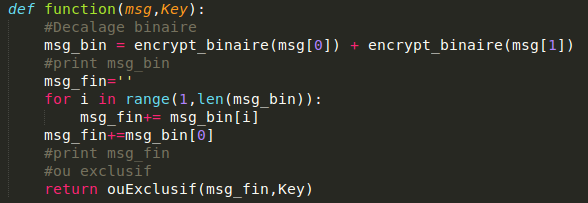
\includegraphics[scale=0.5]{function}
\caption{Fonction de Feistel}
\end{figure}

%------------------------------------------------

\section{Réseau de Feistel}\index{Feistel}

\subsection{Chiffrer}

\paragraph{}Le réseau de Feistel est symbolisé par la fonction \textbf{encrypt\_feistel()} qui à partir d'un bloc et d'une clé, va chiffrer un texte. Tout d'abord, nous divisons le bloc en deux, le bloc gauche et le bloc droit. Pour chaque caractère de la clé (i.e. 4 boucles), nous effectuons les opérations suivantes. On réalise la copie du bloc droit, on prend les deux premier caractères de la clé et on les stocke, on décale la clé de 1 caractère, on transforme le bloc droit à travers la fonction function() à laquelle on lui envoie le bloc droit lui-même ainsi que la clé convertie en binaire. Une fois cela réalisé, on effectue le ou exclusif avec le nouveau bloc droit (résultat de la fonction function()) et la partie gauche. Le résultat obtenu est ainsi converti en caractère, on stocke la copie du bloc droit dans le bloc gauche, et on réitère ce traitement. Nous obtenons finalement notre bloc chiffré à partir de la clé.
\clearpage
\begin{figure}[!h]
\centering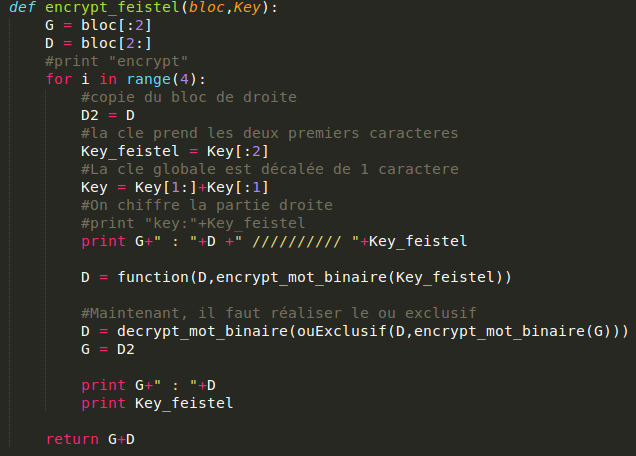
\includegraphics[scale=0.5]{feistel}
\caption{Réseau de Feistel pour chiffrer}
\end{figure}


%------------------------------------------------

\subsection{Déchiffrer}

\paragraph{}Dans l'optique inverse, nous avons conçu \textbf{decrypt\_Feistel()}, qui à partir d'un bloc chiffré et d'une clé va déchiffrer le message. L'opération est similaire à encrypt\_Feistel(), nous divisons notre bloc de 4 caractères en deux blocs : gauche et droite. À la différence de encrypt\_Feistel(), nous parcourons la clé à l'envers (i.e. « XK » → « CX » → « XC » → « KX ») mais nous effectuons les mêmes opérations : le bloc droit passe par function(), puis le résultat obtenu subit un ou exclusif avec le bloc gauche, et finalement on inverse le bloc gauche avec le bloc droit.

\begin{figure}[!h]
\centering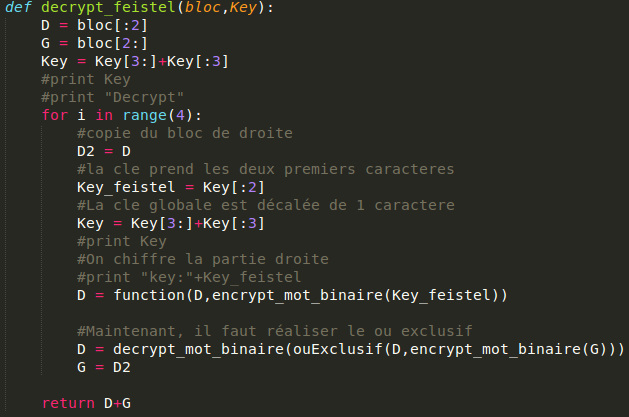
\includegraphics[scale=0.5]{dechiffrement_feistel}
\caption{Déchiffrement par Feistel}
\end{figure}

%------------------------------------------------

\subsection{Exemple}

\paragraph{}Afin d'illustrer un exemple concret de fonctionnement du réseau de Feistel, nous avons procédé à une fonction main() permettant de simuler l'échange d'un texte chiffré.
\vspace{0.5cm}Nous choisissons un mot arbitraire « AAAA??BB » et une clé « KXCX ». Nous nous assurons que les lettres soient en lettres majuscules (mot.upper()). Nous « préparons » le texte de sorte que sa taille soit un multiple de 4 par le fonction tailleTexteMod4() qui va ajouter des espaces à la fin du mot. Par la suite, nous chiffrons bloc par bloc le texte (taille de 4 caractères). Nous obtenons ainsi « MYMWEQG, ». Et en effectuant l'opération inverse par la fonction decrypt\_feistel() nous ré-obtenons « AAAA??BB ».

\begin{figure}[!h]
\centering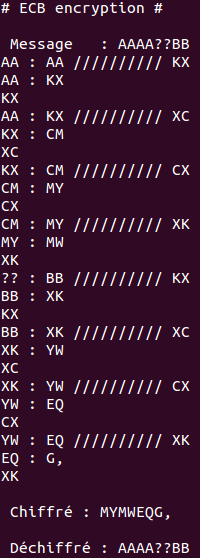
\includegraphics[scale=0.5]{exemple}
\caption{Exemple de chiffrement}
\end{figure}

%------------------------------------------------

\section{Cipher-bloc Chaining}

\paragraph{}Maintenant intéressons nous au chiffrement et déchiffrement en mode CBC. Tout d'abord, nous avons la fonction vecteur\_initialisation() qui va prendre au hasard 4 caractères dans le dictionnaire pour former la clé. Une fois cette clé formée, nous effectuons un ou exclusif avec le texte en clair. Avec le resultat, nous opérons avec la fonction du réseau de feistel. Une fois l'opération terminée, nous recommençons mais en prenant cette fois-ci le résultat de la fonction et le texte en clair.

\begin{figure}[!h]
\centering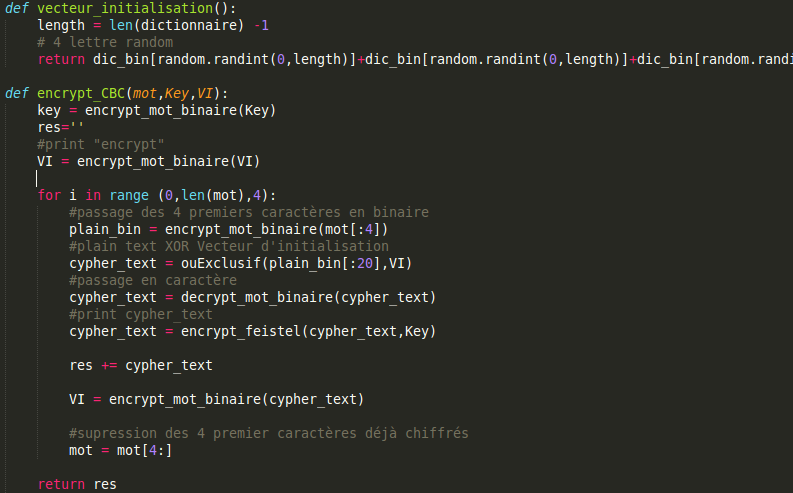
\includegraphics[scale=0.5]{cbc}
\caption{CBC}
\end{figure}

%----------------------------------------------------------------------------------------
%	CHAPTER 2
%----------------------------------------------------------------------------------------

\chapter{TP2 : Cryptographie RSA}

%------------------------------------------------

\section{Introduction}

\paragraph{}Nous avons simulé un échange de messages avec le protocole RSA entre deux identités à l'aide de 3 programmes. Les programmes A et B simulent Alice et Bob, deux personnes souhaitant communiquer de manière secrète, et finalement le programme C représentant l'autorité décernant les clés aux différentes personnes. Nous allons nous intéresser dans un premier temps au programme C qui génère les différentes clés, puis nous étudierons le fonctionnement de l'échange de messages.

%------------------------------------------------

\section{Le programme C}

\paragraph{}La fonction centrale de ce programme est la fonction \textbf{generation()} permettant d'éditer l'ensemble des clés
\\Tout d'abord, nous choisissons 2 nombres premiers aléatoires à l'aide de la fonction \textbf{get\_random()} qui va tirer au hasard un nombre puis va vérifier s'il est premier grâce à la méthode \textbf{lucas\_lehmer()}.
Cette dernière fonctionne ainsi : elle reçoit en paramètre un nombre à tester ainsi qu'un nombre de test qui par défaut est 7. Ce nombre correspond aux nombres de boucles de test que nous réalisons pour tester la primalité du nombre. Tout d'abord si le nombre à tester, que nous appellerons n, est inférieur à 1 le test retourne faux. Ainsi que si n est égal à 2 le test retourne vrai. Nous arrivons dans la boucle principale où le traitement sera réitéré plusieurs fois. En premier lieu nous choisissons un nombre aléatoire entre 3 (car nous excluons 1 et 2) et n-2 . Nous réalisons l’exponentiation modulaire de a\^n-1 mod n. Si le résultat est différent de 1,  on retourne faux. Sinon nous établissons la liste des primitifs de n(cf plus bas la description de la fonction \textbf{primes()}). Nous parcourons cette liste et à chaque primitif nous réalisons a\^(n-1)/q mod n. Si le résultat est égal à 1, nous retournons faux. A la fin de la boucle, si le test n'a retourné aucune valeur, nous finissons par le retour de vrai, car nous avons trouvé que n est un nombre entier.
\\\vspace{0.5cm}Fonction \textbf{primes()}. Cette fonction permet de trouver la liste des entiers primifs d'un nombre entier. Tout d'abord, nous allouons un tableau, et un indice de départ d égal à 2 (premier nombre premier). Nous entrons ensuite dans la boucle while principale où la condition est tant que d² ≤ n , avec n le nombre premier. Dans cette boucle, nous entrons dans une sous-boucle while  où la condition est (n \% d) == 0. Si la condition est respectée, on ajoute d à la liste. Puis on divise n par d, en gardant la partie entière. On sort de la sous-boucle while , on incrémente d et on recommence. Lors de la sortie de la boucle principale while, si n>1 on ajoute n à la liste des entiers primitifs, dans tous les cas on retourne la liste.
\vspace{0.5cm}Retournons à la génération des clés, nous avons grâce aux fonctions précédentes, 2 nombres entiers que nous nommerons p et q. Nous calculons n = p*q puis phi(n) = (p-1)*(q-1). Maintenant nous cherchons e, qui est un nombre premier aléatoire entre 1 et phi(n). Intéressons nous à la fonction e\_aleatoire(phi). Cette fonction tire un nombre premier aléatoire entre 2 et phi-1 uniquement si ce nombre ne possède aucun diviseur commun avec phi.
\vspace{0.5cm}Maintenant que nous possédons la clé privée (i.e. e), nous pouvons éditer la clé publique	. Pour cela 
nous devons chercher d, l'inverse modulaire de phi modulo n. Nous faisons appel à la fonction \textbf{inverse\_modulaire(e,phi)}. Cette fonction utilise l’algorithme suivant :
\begin{itemize}
\item les constantes u0 = 1, u1 = 0, v0=0 et v1 = 1
\item r0 = (e * u0) + (phi * v0)
\item r1 = (e * u1) + (phi * v1)
\item Tant que r1 est différent de 0 nous faisons
	\begin{itemize}
	\item q = r0 / r1
	\item r = r0
	\item u = u0
	\item v = v0
	\item on affecte à r0 la valeur de r1, ainsi que u0 reçoit u1 et v0 vaut v1.
	\item r1 = r – (q * r1)
	\item u1 = u – (q * u1)
	\item v1 = v – (q*v1)
	\end{itemize}

\item Une fois terminé,  nous incrémentons b à u0 afin qu'il devienne positif
\item On retourne u, l'inverse modulaire de phi.
\end{itemize}
\vspace{0.5cm}La fonction génération retourne le couple e,d,n qui comporte clé publique/privée pour le futur utilisateur.

%------------------------------------------------

\section{Le programme A et B}
\paragraph{}Maintenons nous allons étudier le fonctionnement des différents opérateurs dans l'échange de leur message. Nommons les A et B. 
\subsection{Etape 1}
\paragraph{}A souhaite envoyer le message suivant : « AB ?! » vers B. Pour cela il fait appel à la fonction \textbf{envoie\_message\_to\_B(message)} qui va encoder le message selon le protocole RSA. C'est à dire que nous allons convertir chaque caractère en nombre. Pour cela nous réutilisons le dictionnaire du TP précédent. Maintenant que nous avons un nombre, nous effectuons le calcul suivant : 
\\soit M le nombre à chiffrer et (d,n) la clé publique de B
\\C = M\^d mod n
\vspace{0.5cm}Nota Bene : à des fins pratiques, nous utilisons la fonction d'exponentiation modulaire rapide pour limiter l'utilisation du processeur et pour une résultat plus rapide.
\vspace{0.5cm}Une fois notre nombre chiffré, nous recommençons avec les autres caractères du message. Ce qui nous donne une liste de nombres. Nous envoyons cette liste à B qui va commencer le déchiffrement.
\\Pour cela, B utilise \textbf{decrypt\_message\_from\_A(msg\_crypt)} . Cette fonction va prendre chaque nombre dans la liste reçue et le déchiffrer en utilisant la formule suivante : 
\\soit C le message chiffré, (e,n) la clé privée de B
\\M = C\^e mod n
\subsection{Etape 2}
\paragraph{}Une fois le message lu, B compare si le message reçu est égal à « AB?! ». Si tel est le cas, B prépare le message « AB OK » pour A. Il le chiffre de la même manière que A en faisant C = M\^d mod n avec ( d,n) la clé publique de A.
\vspace{0.5cm}A reçoit le message, le déchiffre et le compare à « AB OK ». S'ils sont similaires, on passe à l'étape 3

\subsection{Etape 3}
\paragraph{}A génère 4 caractères aléatoires à partir de son dictionnaire. Puis il les envoie à B en utilisant le protocole RSA.  B les déchiffre, puis les chiffre pour les renvoyer à A. A son tour, A déchiffre pour vérifier que le message a bien été reçu.

\subsection{Etape 4}
\paragraph{}Puisque A et B possède le même mot de passe, on va pouvoir effectuer les opérations suivantes. On effectue le ou exclusif de « AB OK » et du mot de passe. Puisque que le message possède une taille plus grande que le mot de passe ( 4 caractères contre 5), nous nous sommes adaptés à la fonction ouExclusif(). En effet nous effectuons un ou exclusif uniquement avec les caractères nécessaires en partant de la droite du message. \\Exemple :
\vspace{0.5cm}AB OK → message
\\ABCD → mot de passe
\\Nous alignons à droite le mot de passe
\vspace{0.5cm}AB OK
\\ABCD
\\puis nous découpons le messages
\\B OK
\\ABCD
\\Maintenant nous effectuons un ou exclusif de B OK et ABCD.
\\Puisque le XOR de A et 0 donne A, nous prenons A et ajoutons le résultat du XOR à la suite.

\subsection{Etape 5}
\paragraph{}Avec notre mot de passe ainsi généré ( la clé pour le réseau de Feitel), nous pouvons commencer le chiffrement. Nous avons adapté la fonction \textbf{encrypt\_feistel} en \textbf{encrypt\_feistel\_2}  , elle permet de réaliser le chiffrement avec des tailles différentes de 4 caractères. A chiffre son message puis l'envoie à B qui va le déchiffrer avec le même mot de passe(clé). 

\begin{figure}[h]
\centering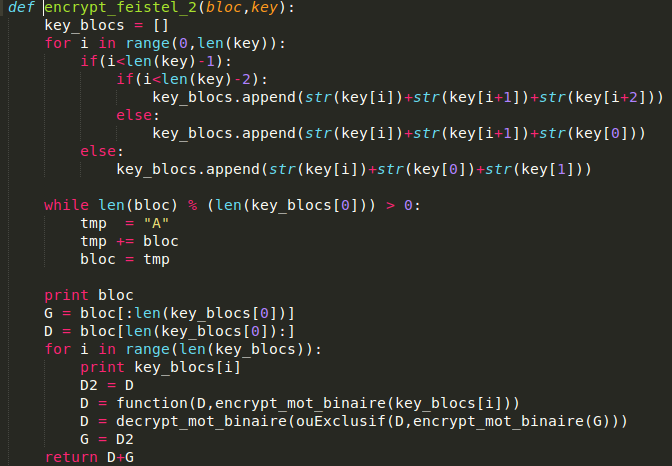
\includegraphics[scale=0.5]{encrypt_feistel2}
\caption{Nouvelle version du réseau de Feistel}
\end{figure}

\end{document}